%%% Laboratory	 Notes
%%% Template by Mikhail Klassen, April 2013
%%% Contributions from Sarah Mount, May 2014
\documentclass[a4paper]{tufte-handout}

\newcommand{\workingDate}{\textsc{May $|$ 2014}}
\newcommand{\userName}{Your Name}
\newcommand{\institution}{Your University}

\usepackage{lab_notes}
\usepackage{listings}
\usepackage{color}
\usepackage{hyperref}
\hypersetup{
  pdffitwindow=false,            % window fit to page
  pdfstartview={Fit},            % fits width of page to window
  pdftitle={Lab notes 2014},     % document title
  pdfauthor={Your Name},         % author name
  pdfsubject={},                 % document topic(s)
  pdfnewwindow=true,             % links in new window
  colorlinks=true,               % coloured links, not boxed
  linkcolor=DarkScarletRed,      % colour of internal links
  citecolor=DarkChameleon,       % colour of links to bibliography
  filecolor=DarkPlum,            % colour of file links
  urlcolor=DarkSkyBlue           % colour of external links
}


\title{Tech Notes}
\date{2017}

\begin{document}
\maketitle

\newday{23 July 2017}
Chaper 1
\begin{projects}
  Symbol Table
  \begin{itemize}
  \item it is a data structure maintained by compiler
  \item store names of all entities
  \item verify if a veriable has been declared
  \item determine the scope of a name
  \item used to realize type checking
  \end{itemize}

  \begin{itemize}
  \item Declaration introduces the name and type of a variable so that the compiler knows what the name means if it occurs later in the program.
  \item Variable Definition causes the compiler to reserve a memory block of appropriate size to hold the value of the variable.
  \end{itemize}

  Declaration and Definition
  \begin{lstlisting}[language=C]
    int a;//definition and declaration
    extern int a;//declaration
    int b = 1;//definition and declaration
  \end{lstlisting}
\end{projects}

Constants
\begin{enumerate}
\item Constants are variables that value never change. They are called immutable.
\item As a convention, always name constants with UPPER\_SNAKE\_CASE;
\end{enumerate}

Naming Convention
\begin{itemize}
\item Camel case: words seperated by initial capital letter (camelCase or CamelCase).
\item Snake case: words seperated by underscore (snake\_case or SNAKE\_CASE).
\item Variable and functions: camel case with lower case first letter. avgInvest...
\item Constancs: all captial snake case.
\item Type and class: camel case with uppercase first letter. StockContainer...
\end{itemize}

Operator
\begin{itemize}
\item Discuss that the assignment operator yields as a value the value being assigned, but the main purpose is the side-effect that a the value is assigned to the variable.
\item Discuss that for <<, the main purpose is the side effect (i.e., inserting the data into the stream). And yes, it yields a stream as a value that is needed for chaining.
  \begin{lstlisting}[language=C]
    if(a = 0)...//false
    if(a = 1)...//true
  \end{lstlisting}
\item Caution! If all the operands are integers then integer division is performed, any fractional part is automatically discarded!
  \begin{lstlisting}[language=C]
    double tempF = tempC * 9 / 5 + 32;//loss precision
    double tempF = tempC * 9.0 / 5 + 32;//accurate
  \end{lstlisting}
  \begin{lstlisting}[language=c]
    bsl::cout << ``Hello'' << name << ``\n'';
    effectively is (((bsl::cout << ``Hello'' ) << name) << ``\n'');
    Explain that a = b = c= 123;
    is the same as a = ( b = ( c = 123; ) )
  \end{lstlisting}
  This introduces an example of an operator that is right associative.Also, this explain why an assignment returns bthe value that it assigns.
\end{itemize}

Basic input and output

\begin{enumerate}
\item C++ uses streams to abstract input and output
  Streams can represent the screen, keyboard, a file, etc.
\item Streams are used to either insert or extract characters
  They represent a source or destination
  Characters are handled sequentially, one after the other
\item bsl::endl is a stream manipulator that inserts a newline character
  \begin{itemize}
  \item But also requests the data is physically written to the destination (called flushing).
  \item Flushing is usually expensive and streams have optimisations to minimise it
  \end{itemize}
\item
\end{enumerate}

%%%%%%%%%%%%%%%%%%%%%%%%%%%%%%%%%%%%%%%%%%%%%%%%%%%%%%%%
\newday{July 26th 2017}
Bash

command + \& -> run in background \newline
shell define vaiable without \$, access variable with \$.
quote stop match regular expression but does not stop variable access.

Vim\newline
x - delete char\newline
5x - delete 5 chars\newline
dd - delete a whole line \newline
5dd - delete 5 lines \newline
dw - delete a word \newline
5dw - delete 5 words \newline
shift + char - capital char (also valid in Emacs) \newline
cw - change word \newline
. - repeat last command \newline
cc - change the entire line \newline
\$ end of line, \^ beginning of line \newline
:+10 :-5 move cursor according to line number \newline

C++\newline
main can't be put in a namespace or the compiler won't find it because it won't be main in the symbol table but with some extra prefix related with the namespace.\newline
a() + b() + c(), specific evaluation sequence is not defined before C++11.\newline
reference much be initialized, pointer could point to null.
%%%%%%%%%%%%%%%%%%%%%%%%%%%%%%%%%%%%%%%%%%%%%%%%%%%%%%%%
\newday{July 27th 2017}

\textbf{GIT}
\begin{enumerate}
\item The stage is used for telling Git what to care about in future commands.
\item To remove files from stage : git reset  HEAD [path] e.g.\ git reset HEAD readme.md
\item Commit creat a snapshot in history of all files
\item Supplies a unique hash used for referring to the moment in histroy
\item To keep files but remove Git tracking : git rm --cached [file]
  \begin{itemize}
  \item --cached tells Git to remove tracking on this file, but keep local file.
  \item git rm [file] remove local
  \end{itemize}
\item A fork creates a remote repository by cloning
\item Use pull request to merge changes in fork back to its parent repository.
\item Note that each commit hash actually reference a complete snapshot of the repository. The snapshot contains a commit hash for EVERY FILE.
\item remote remote branch git push origin :{branch-name} \footnote {Pay attention to the space positon}
\item Fast forward merg happen only if history has not diverged
  \item merge order, merge master on current branch, checkout to master and merge local feature branch, push master, delete local branch
\end{enumerate}
\begin{maybe}
  \begin{itemize}
  \item Reimplement the ideas from the paper \textit{Getting Reference Counting Back in the Ring} \citep{Shahriyar+12}
  \end{itemize}
\end{maybe}

%%%%%%%%%%%%%%%%%%%%%%%%%%%%%%%%%%%%%%%%%%%%%%%%%%%%%%%%

\newday{August 3rd 2017}
class object data member initialization sequence is exactly as they are declared in the private domain.
rvalue could not be referenced because they can't be addressed;
\begin{lstlisting}[language=c++]
this[0].name equals this->name
\end{lstlisting}

%%%%%%%%%%%%%%%%%%%%%%%%%%%%%%%%%%%%%%%%%%%%%%%%%%%%%%%%
\newday{August 7th 2017}
pass pointer essentially pass a pointer value to local variable in a function, in this way, the pointer value points to the same place. But the pointer variable's address is different.

const is a contract made with compiler -- compiler level restriction.
\begin{lstlisting}[language=C++]
  const int DAYS = 7;//compiler knows days is integer
  #define DAYS 7 // compiler doesn't see the DAYS, string replaced by proprecessor.
\end{lstlisting}
\textcolor{red}figure out reference assignment such as:
\begin{lstlisting}[language=C++]
  int& t = foo();
\end{lstlisting}
Class constructor use explicit when it only has one argument - to avoid implicit conversion.

always use getter and setter in design.

Static member is also a class member. It could access class data members.

\textcolor{red}{figure out return mechanism}
\textcolor{blue}{cin stream will stop every time face a blank}
%%%%%%%%%%%%%%%%%%%%%%%%%%%%%%%%%%%%%%%%%%%%%%%%%%%%%%%%
\newday{August 9 2017}
when function returns the return value is passed to EAX register, the local variable is gone.
EAX is used for assignment.
\begin{lstlisting}[language=C++]
  int a = foo();
\end{lstlisting}
%%%%%%%%%%%%%%%%%%%%%%%%%%%%%%%%%%%%%%%%%%%%%%%%%%%%%%%%
\newday{August 10 2017}
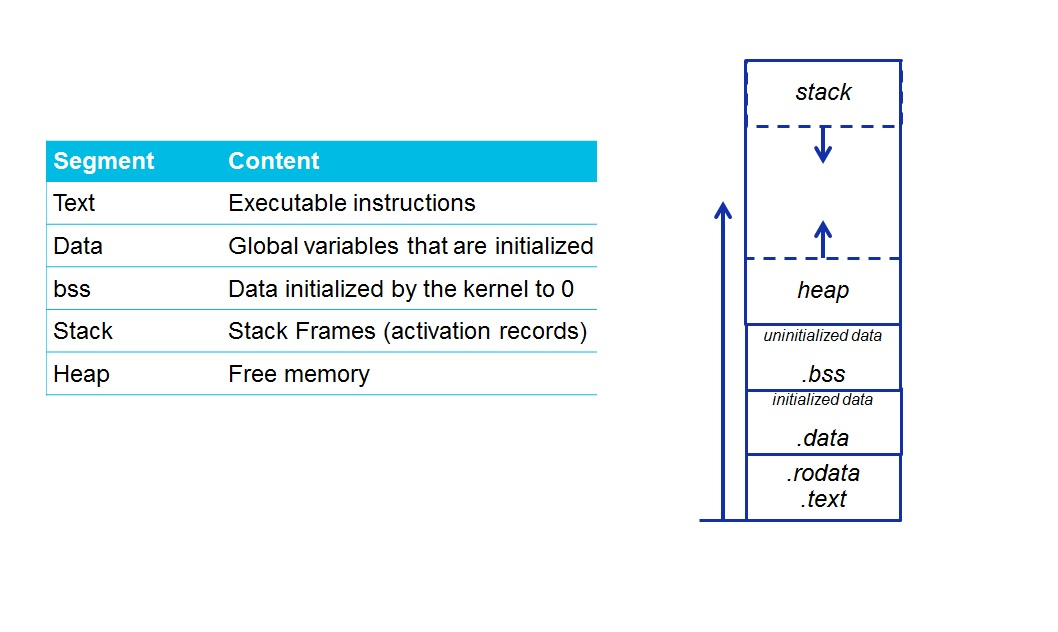
\includegraphics[scale=0.65]{memory.jpg}
arr[5] is a syntax suger for *(arr+5).\newline
There is no simple corresponding way to allocate a multi-dimensional array dynamically, you have to allocate an array of pointers, and then allocate each row\'s worth of elements individually.

%%%%%%%%%%%%%%%%%%%%%%%%%%%%%%%%%%%%%%%%%%%%%%%%%%%%%%%%
\newday{August 30 2017}
%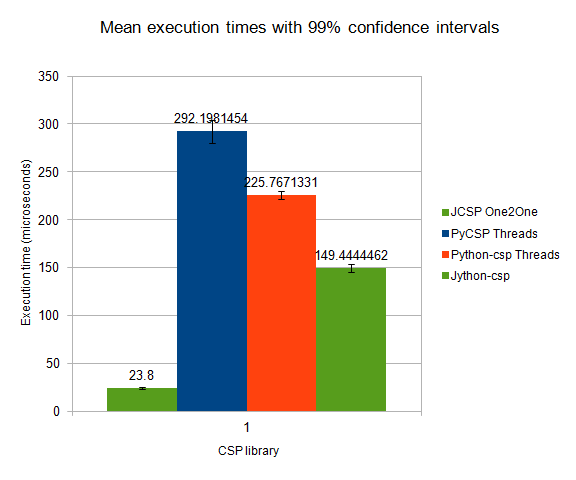
\includegraphics[scale=0.65]{benchmark}
cppflags is used by complier
complier implicit does \$(CC) \$(CPPFLAGS) \$(CFLAGS) -c -o \$@ \$<
\begin{lstlisting}[language=c++]
#include <iostream>
class Base {
  public:
    void foo() {std::cout << "base foo called\n";}
};

class Derived : public Base {
  public:
    Derived(const char* a) {
        std::cout << "Derived constructor\n";
        std::cout << a << std::endl;
    }
    void foo() {std::cout << "Derived foo called\n";}
};

int main(){
    Derived d("i am d\n");
    d.foo();
    return 0;
}
\end{lstlisting}
comcrete function in base and derived class.
%%%%%%%%%%%%%%%%%%%%%%%%%%%%%%%%%%%%%%%%%%%%%%%%%%%%%%%
\newday{August 31, 2017}
Google mock a abstract class:
\begin{lstlisting}[language=c++]
  const Forward* somefunc(int a) const;
  MOCK\_CONST\_METHOD(somefuck, const Forward*(int))
\end{lstlisting}
\textcolor{red}{without tailing const}

%%%%%%%%%%%%%%%%%%%%%%%%%%%%%%%%%%%%%%%%%%%%%%%%%%%%%%%
\newday{September 5, 2017}

%%%%%%%%%%%%%%%%%%%%%%%%%%%%%%%%%%%%%%%%%%%%%%%%%%%%%%%%
\newday{September 7, 2017}
In Bloomberg:
Google\_Mock need to include IS\_GMOCK\_MAIN=yes\\
makefile srcdirs need to specify the very folders, you can't assume it look for source files recursively.\\
If makefile srcdirs specified, excludesrcfile key word doesn't take effect.
%\newpage

%%%%%%%%%%%%%%%%%%%%%%%%%%%%%%%%%%%%%%%%%%%%%%%%%%%%%%%%
\newday{September 17, 2017}
systemctl stop mariadb.service\\
systemctl start mariadb.service\\
%必须以root用户登录myriadb才可以创建用户:\\
mysql -u root -p\\
CDtnsl17\\
CREATE USER 'YanMac'@'%' IDENTIFIED BY 'passw0rd';\\
grant all PRIVILEGES on *.* to YanMac@'%' identified by 'passw0rd'; %//给YanMac用户在任何dining上用‘passw0rd’登录的权限;\\
%%%%%%%%%%%%%%%%%%%%%%%%%%%%%%%%%%%%%%%%%%%%%%%%%%%%%%%%
on mac, mysql.server start

\newday{September 23, 2017}
\begin{lstlisting}[language=c++]
  namespace std {
    class Node {
      public:
      Node(string name):d_name(name), d_children() {}
      string& name(){ return d_name;}
      const string& getName() const {return d_name;}
      set<Node>& children() { return d_children;}
      private:
      string d_name;
      set<Node> d_children;
    };

    inline bool operator<(const Node& lhs, const Node& rhs) {
      return lhs.getName() < rhs.getName();
    }

  }//close std

\end{lstlisting}
In this, why inline could solve the duplication error??

\textcolor{red}{How to use unordered\_set with customized hash??}
\newday{September 27, 2017}
\begin{itemize}
\item C++ complier makes default constructor, default assignment operator, default copy constructor by necessity. Only if there are such operations in the code, correspondent component would be generated. Declared these as private to forbid using them.\\
\item If you want to use [] to access element in C++ map, the value type should support default constructor.
\end{itemize}

\newday{September 28, 2017}
If there is a virtual function in class, you need to make the destructor virtual.
Each class maintains a vtable about different virtual function.

\newday{October 4, 2017}
\begin{lstlisting}[]
  latexmk -pdf compile latex file.
  xelatex cv.tex compile with xelatex mode.
\end{lstlisting}

\newday{October 8, 2017}
\begin{lstlisting}
open mysql:mysql.server start
\end{lstlisting}

\newday{October 10, 2017}
ecs git sync fail because ssh-agent not set up.\\

\begin{lstlisting}
Start the ssh-agent in the background.
eval "$(ssh-agent -s)"
Agent pid 59566
ssh-add private key file
push/pull
\end{lstlisting}

\newday {October 12, 2017}
\begin{itemize}
\item In python, parameters are passed by reference.
\item dictionary elements could be poped by key
\item , character after print means next print output keep on the same line print a, b
\item object is the mother of all classes in Python. class classname(object)
\item use is to compare whether variables' identity which means whether they refer to the same object, use == to compare whether their values are equal.
\item two demensional array can\'t be initialized by * like  multi = [[0] * 5] * 3
  should be initialized via  [[0 for col in range(5)] for row in range(3)]
\item python would load lib of xxx.pyc first, if you wanna load from another place, remove this file
\item python 2 don\'t allow children function modify upper level local variable, in Python 3, nonlocal keyword is induced to solve this problem.
  \item Queue.Queue and collections.deque serve different purposes. Queue.Queue is intended for allowing different threads to communicate using queued messages/data, whereas collections.deque is simply intended as a datastructure. That\'s why Queue.Queue has methods likeput\_nowait(), get\_nowait(), and join(), whereas collections.deque doesn\'t. Queue.Queueisn\'t intended to be used as a collection, which is why it lacks the likes of the in operator.
It boils down to this: if you have multiple threads and you want them to be able to communicate without the need for locks, you\'re looking for Queue.Queue; if you just want a queue or a double-ended queue as a datastructure, use collections.deque.
Finally, accessing and manipulating the internal deque of a Queue.Queue is playing with fire - you really don't want to be doing that.
\end{itemize}

\newday{10/29/2017}
In c++, if you wanna define a in class const variable. Generally you could do it in 2 ways:
\begin{lstlisting}[language=c++]
class X {
	static const int c1 = 7;
	enum { c2 = 19 };

	char v1[c1];
	char v2[c2];

	// ...
};

class Y {
  public:
    Y():i1(2) {}
  private:
    const int i1;
};
initialize const variable in constructor;
\end{lstlisting}
A class is typically declared in a header file and a header file is typically included into many translation units. However, to avoid complicated linker rules, C++ requires that every object has a unique definition. That rule would be broken if C++ allowed in-class definition of entities that needed to be stored in memory as objects.\\
\textbf{Why are only static const integral types \& enums allowed In-class Initialization?}

The answer is hidden in Bjarne\'s quote read it closely,
"C++ requires that every object has a unique definition. That rule would be broken if C++ allowed in-class definition of entities that needed to be stored in memory as objects."

Note that only static const integers can be treated as compile time constants. The compiler knows that the integer value will not change anytime and hence it can apply its own magic and apply optimizations, the compiler simply inlines such class members i.e, they are not stored in memory anymore, As the need of being stored in memory is removed, it gives such variables the exception to rule mentioned by Bjarne.

It is noteworthy to note here that even if static const integral values can have In-Class Initialization, taking address of such variables is not allowed. One can take the address of a static member if (and only if) it has an out-of-class definition.This further validates the reasoning above.

enums are allowed this because values of an enumerated type can be used where ints are expected


\bibliographystyle{plain}
\bibliography{lab_notes}
\end{document}
